%% Please fill in your name and collaboration statement here.
\newcommand{\studentName}{Kevin Zhang}
\newcommand{\collaborationStatement}{I worked with Tomoya Hasegawa and Annie Hwang, got help from no one else, and referred to no other resources.}


%%%%%%%%%%%%%%%%%%%%%%%%%%%%%%%%%%%%%%%%%%%%%%%
\documentclass[solution, letterpaper]{cs121}
\usepackage{enumerate}
\usepackage{enumerate}
\usepackage{tikz}
\usepackage{pgf}
\usepackage{tikz}
\usetikzlibrary{arrows,automata}
\usepackage{hyperref}
\usetikzlibrary{automata,positioning}

\begin{document}
\header{3}{Tuesday October 6, 2015 at 11:59pm}
%%%%%%%%%%%%%%%%%%%%%%%%%%%%%%%%%%%%%%%%%%%%%%%
\PART{Varun and Erin}
%%%%%%%%%%%%%%%%%%%%%%%%%%%%%%%%%%%%%%%%%%%%%%%


\problem{3+3+3+3+3} {3/4 page}
For each of the following languages, state whether the language is regular or non-regular. If regular, state a regular expression that denotes the language. If non-regular, write a short proof to justify.

\subproblem \{$xyx^R : x, y \in \Sigma^*$ \}
\subproblem \{$a^ib^ja^jb^i$: $i$, $j\geq0$\}.
\subproblem
$\{w\;:\;\textrm{$w$ is, for some $n\geq 1$, the decimal notation
for $10^n$}\}$. 
\subproblem $\{a^{2n}b^{n}: n\geq 0\}$
\subproblem $\{a^nb^n : n \geq 0$ and $n \neq 3i+5j$ for any $i \in \mathbb{N}, j \in \mathbb{N} \}$ Hint: Try explicitly working out all the strings in the language.

\begin{solution}
\subsolution $\Sigma^*$ consists of any string, including the empty string $\vareps$.  Then it's easy to see that any string is in this language simply by choosing $x = \vareps$, because then the result is just $y$, which can represent any string.  Although this is a trivial proof, any string can definitely be represented in this fashion, just by examining the beginning and end of the string for matching reverse strings and letting those be $x$ and $x^R$.  This is a regular language, given by $\Sigma^*$.
\subsolution Use the standard proof for disproving regularity using contradiction.  In general, this type of proof involves assuming that the given language is regular, then proving that some set of inputs results in an infinite number of states in the DFA representing that regular language.  Since DFAs can only have a finite number of states, this is a contradiction; hence, the given language cannot be represented by a DFA, and therefore cannot be regular.  
\\\indent Our proof consists of proving that there is an infinite number of states in the DFA; the remaining part of the proof is detailed above.  Consider two distinct pairs of natural numbers $i_1,j_1$ and $i_2,j_2$.  Then D must end in different states after receiving either pair of inputs $a_{i_1}b_{j_1}$ or $a_{i_2}b_{j_2}$.  If D ends in the same state for these two pairs of inputs, then, since $a_{i_1}b_{j_1} \cdot b_{i_1}a_{j_1}$ ends in a final state, so does $a_{i_2}b_{j_2} \cdot b_{j_1}a_{i_1}$.  But this is a contradiction, since $(i_1,j_1) \neq (i_2,j_2)$ and therefore the second string cannot be in the given language.  Hence, every pair of inputs $a_ib_j$ must result in a different state in D.  Therefore, based on the assumption of regularity, D has an infinite number of states, an impossibility.
\subsolution This is just $10(0)^*$.
\subsolution This is no different from $(aa)^nb^n$, which is the exact format of the archetypal non-regular language.
\subsolution This is regular because this language is finite; $n$ has a maximum, according to the Chicken McNugget Theorem (a real thing, I promise!) which states that the maximum integer that cannot be written in the form $ai + bj$ for any $i, j \in \mathbb{N}$ is $ab - a - b$.  The actual regular expression is $\vareps \cup ab \cup a^2b^2 \cup a^4b^4 \cup a^7b^7$.
\end{solution}

\problem{2+4} {1/2 page}

\subproblem
A context-free grammar $G$ is ambiguous if there exists a
string $w \in L(G)$ with two distinct leftmost derivations in $G$. Show that the context-free grammar $G = (V, \Sigma, R, S)$, where
$V=\{S,A\}$, $\Sigma = \{a,b\}$, and $R = \{S \rightarrow AA, A
\rightarrow AAA, A \rightarrow bA, A \rightarrow Ab, A \rightarrow a\}$
is ambiguous, because $aba$ has two different leftmost derivations in 
$G$.

\subproblem
Prove that $L(G)$,
where $G$ is the context-free grammar in Part (A), is regular.


\begin{solution}
\subsolution This left-most derivation,

\begin{center}
\begin{tikzpicture}[shorten >=1pt, node distance = 1cm, on grid, auto] 
	\node 	(S) 							{$S$};
	\node 	(A1) 	[below=of S, xshift=-2cm] 		{$A$};
	\node 	(A2) 	[below=of S, xshift= 2cm]		{$A$};
	\node	(A3)	[below=of A1, xshift=-1cm]		{$A$};
	\node 	(b)	[below=of A1, xshift= 1cm]		{$b$};
	\node	(a1)	[below=of A3]				{$a$};
	\node	(a2)	[below=of A2]				{$a$};

	\path [->, line width=1pt]
	(S)	edge 	node {} 	(A1)
		edge		node {}	(A2)
	(A1)	edge		node {}	(A3)
		edge		node {}	(b)
	(A3)	edge		node {}	(a1)
	(A2)	edge		node {}	(a2)
	;

\end{tikzpicture}
\end{center}

and the left-most derivation,

\begin{center}
\begin{tikzpicture}[shorten >= 1pt, node distance = 1cm, on grid, auto]
	\node	(S)							{$S$};
	\node	(A1)	[below=of S, xshift=-2cm]		{$A$};
	\node	(A2)	[below=of S, xshift= 2cm]		{$A$};
	\node	(b)	[below=of A2, xshift=-1cm]		{$b$};
	\node	(A3)	[below=of A2, xshift= 1cm]		{$A$};
	\node	(a1)	[below=of A1]				{$a$};
	\node	(a2)	[below=of A3]				{$a$};
	
	\path [->, line width=1pt]
	(S)	edge		node {}	(A1)
		edge		node {}	(A2)
	(A1)	edge		node {}	(a1)
	(A2)	edge		node {}	(b)
		edge		node {}	(A3)
	(A3)	edge		node {}	(a2)
	;
\end{tikzpicture}
\end{center}

\end{solution}

both result in the same expression, $aba$.

\subsolution Because this isn't a left-or right-regular language, it's difficult to say whether this is regular or not.  Thus, we can only do a holistic analysis.  Note that every $A$ eventually becomes a small $a$, while every $A$ can also become $Ab$ or $bA$ at any point.  This tells us that we can insert a $b$ anywhere.  Note moreover that the number of total number of $A$'s only ever increases by even amounts; this tells us that the total number of $a$'s is even.  Thus, this CFG describes any string that contains a positive, even number of $a$'s.  The last part to determine is whether this is a regular language; the expression $(b^*ab^*a)(b^*ab^*a)^*b^*$ is exactly what we want.

\problem{3+3+2}{3/4 page}
$$ L_1 = \{a^nb^m : m,n \geq 0 , m \neq n\} $$
$$ L_2 =  \{a^nb^ma^mb^n : m,n \geq 0\} $$


\subproblem Construct a context-free grammar $G_1$ for $L_1$
\subproblem Construct a context-free grammar $G_2$ for $L_2$.
\subproblem Construct a context-free grammar for $L_1L_2$.

\begin{solution}
Let $S$ be the start state in 

\subsolution Let $V = \{S, A, B\}$, $\Sigma = \{a, b\}$, and $R$ given by the following:
\begin{itemize}
	\setlength\itemsep{0pt}
	\item $S \mapsto aA$
	\item $S \mapsto Bb$
	\item $A \mapsto aA$
	\item $A \mapsto aAb$
	\item $A \mapsto \vareps$
	\item $B \mapsto Bb$
	\item $B \mapsto aBb$
	\item $B \mapsto \vareps$
\end{itemize}

\subsolution Let $V = \{S, A, B\}$, $\Sigma = \{a, b\}$, and $R$ given by the following:
\begin{itemize}
	\setlength\itemsep{0pt}
	\item $S \mapsto A$
	\item $A \mapsto aAb$
	\item $A \mapsto B$
	\item $B \mapsto bBa$
	\item $B \mapsto \vareps$
\end{itemize}

\subsolution Simply combine the above two CFGs.  Let $V = \{S, A, B, C, D, E\}$, $\Sigma = \{a, b\}$, and $R$ given by the following:
\begin{itemize}
	\setlength\itemsep{0pt}
	\item $S \mapsto AD$
	\item $A \mapsto aB$
	\item $A \mapsto Cb$
	\item $B \mapsto aB$
	\item $B \mapsto aBb$
	\item $B \mapsto \vareps$
	\item $C \mapsto Cb$
	\item $C \mapsto aCb$
	\item $C \mapsto \vareps$
	\item $D \mapsto aDb$
	\item $D \mapsto E$
	\item $E \mapsto bEa$
	\item $E \mapsto \vareps$
\end{itemize}
\end{solution}

%%%%%%%%%%%%%%%%%%%%%%%%%%%%%%%%%%%%%%%%%%%%%%%
\PART{Madhu and Serena}
%%%%%%%%%%%%%%%%%%%%%%%%%%%%%%%%%%%%%%%%%%%%%%%
\problem{$3+3+(2)$}{$\frac12$ page}
An \emph{arithmetic progression} is a set of the form $\{p+qn \,:\, n \in \Nat\}$ for some $p,q \in \Nat$. For example, the set $\{10,13,16,19,\ldots\} = \{10+3n \,:\, n \in \Nat\}$ is an arithmetic progression.

\subproblem  Show that if $L \subseteq a^*$ and $\{|w| \,:\, w \in L\}$ is an arithmetic progression, then $L$ is regular. (An example of such a language $L$ is the language $\left\{a^{10+3n} \,:\, n \in \Nat\right\}$.)

\subproblem Use a counterexample to show that if $L \subseteq \{a,b\}^*$ and $\{|w| : w \in L\}$ is an arithmetic progression, then $L$ need not be regular.

\subproblem (Challenge!! Not required; worth up to 2 extra credit points.) Let $S \subseteq \Nat$ be an infinite set that does not contain any arithmetic progression as a subset. Let $L$ be an infinite language and $L \subseteq \{w \in \Sigma^* \,:\, |w| \in S\}$. (In other words. $\forall w \in L$, $|w| \in S$.) Prove that $L$ is not regular.\\\\
\textit{Note: On every problem set we will provide a challenge problem, generally significantly more difficult than the other problems in the set, but worth only a few points. It is recommended that you attempt these problems, but only after completing the rest of the assignment.}

\begin{solution}
\subsolution Let the arithmetic progression of values for $|w|$ be given by $p + qn$.  Since strings in $L$ consists only of $a$, strings in $L$ are therefore exactly $p + qn$ $a$'s in a row for some $p, q, n \in \mathbb{N}$.  Then $L$ is given by the language $L = \{a^{p+qn}: n \in \mathbb{N}\}$.
\subsolution Consider the archetypal non-regular language, $L = \{a^nb^n\}$.  Strings in this language are of even length, which actually are an arithmetic sequence by themselves.  Yet $L \subseteq \{a,b\}^*$, but is not regular; this is a counterexample.
\subsolution This is one case where the pumping lemma comes in very handy.  Suppose the given language $L$ is regular.  Let's take some string $s \in L$.  The pumping lemma tells us that $s$ can be written as $xyz$ where $|y| \ge 1$; moreover, all strings of the form $xy^nz$ where $|n| \ge 1$ are also in $L$.  But this is a contradiction, since the set of strings $xy^nz$ have lengths which form an arithmetic sequence; i.e. there is a subset of strings of $L$ whose string lengths form an arithmetic sequence.  But this contradicts the definition of $S$ and $L$!  Therefore, $L$ cannot be regular.
\end{solution}





\problem{4}{$\frac14$ page}
Define an \emph{arithmetic function} as any function $\Nat \to \Nat$. Use a diagonalization argument to prove that the set of arithmetic functions is uncountably infinite.

\begin{solution}
Suppose the set of arithmetic functions is countable.  Every arithmetic function only sends natural numbers to natural numbers, so if $f$ is an arithmetic function, it is possible for us to list the outputs of $f$ by writing $f(0), f(1), f(2), \cdots$.
Since we assumed the set of arithmetic functions is countable, let's number them $f_0, f_1, f_2, \cdots$, and their outputs for the natural numbers $\{f_{0,0},f_{0,1},f_{0,2}\cdots\}, \{f_{1,0},f_{1,1},f_{2,1},\cdots\}, \cdots$.  (Imagine a table where the columns are the functions and the rows are the natural numbers).  Construct a new function by taking $f(i) = f_{i,i}+1$ for all $i \in \mathbb{N}$.  Note that this function differs from $f_i$ in the $i$th place for all $i \in \mathbb{N}$, meaning that this is an entirely new arithmetic function.  But then this is a contradiction, since we've already listed all arithmetic functions in the table; hence, the set of arithmetic functions cannot be countable, and we are done.
\end{solution}


\problem{4+2}{1/2 page}

Let $\Sigma$ be some alphabet. Consider $L = \{ R : R \text{ is a regular expression for a language over} \Sigma \}$. 

\subproblem Prove that L is not a regular language. 
\subproblem Give a context-free grammar which generates L. 
 
\begin{solution}
\subsolution To do this, we prove that each of the strings in $(^*$ (a string consisting only of left parentheses) must end in different states in any FA that accepts this language.  Note that the given set is just a set of strings, where each string represents a regular expression and the alphabet is $\Sigma \cup \{\cup, (, ), *\}$.
\\\indent Suppose that the above set is a regular language; then there is an FA, $F$, that accepts this language exactly (we don't care whether it's an NFA or a DFA, the result is the same).  Then consider these two expressions: $(^na)^n$ and $(^{n+1}a)^n$, where $n \in \mathbb{N}$.  That is, the expression consisting of $n$ sets of parentheses surrounding an $a$ vs. almost the same expression, but with an extra $($ on the left side.  Note that the first expression is a regular expression, but the second is not because it contains an improper number of parentheses.  Suppose that we feed both $(^n$ and $(^{n+1}$ into $F$.  We claim that no path for these two strings in $F$ end in the same state; if they did, then that implies that $F($ $(^n$ $) = F($ $(^{n+1}$ $) \Rightarrow F($ $(^na)^n$ $) = F($ $(^{n+1}a)^n$ $)$.  This is a contradiction, because the LHS of the second equation is a final state, while the RHS is a non-final state; the equation implies that the two strings in question both are accepted or both are not accepted, which is obviously not true.  Thus, we have proved that all pairs of strings $(^n$ and $(^{n+1}$ end in a different state when fed into $F$.
\\\indent We can extend this logic to any pair of strings $(^m$ and $(^n$; the result is the same.  This tells us that there must be an infinite number of states in $F$, a contradiction!  Thus, there can be no finite automata that accepts $L$, and we are done.

\subsolution A grammar which generates $L$ is given by $V^g = \{S^g, A\}$, $\Sigma^g = \Sigma \cup \{\cup, (, ), *\}$, and $R^g$ given by:
\begin{itemize}
	\setlength\itemsep{0pt}
	\item $S^g \mapsto A$
	\item $A \mapsto A^*$
	\item $A \mapsto (A)$
	\item $A \mapsto AA$
	\item $A \mapsto A \cup A$
	\item $A \mapsto t, t \in \Sigma$ (NOT $\Sigma^g$)
\end{itemize}
where the start is given by $S^g$.
\end{solution}

\problem{6}{1/2 page}
An {\em All-Paths-NFA} is exactly the same as an NFA except 
that it is defined to accept a string $x$ only if {\em all} computation 
paths on $x$ end in an accept state and rejects $x$ otherwise. 
(In contrast, a standard NFA accepted a string if {\em any} 
computation path leads to an accepting state). Show that a language 
$L$ 
is regular if and only if it is recognized by some All-Paths-NFA. 

For example, given the NFA:
\begin{center}
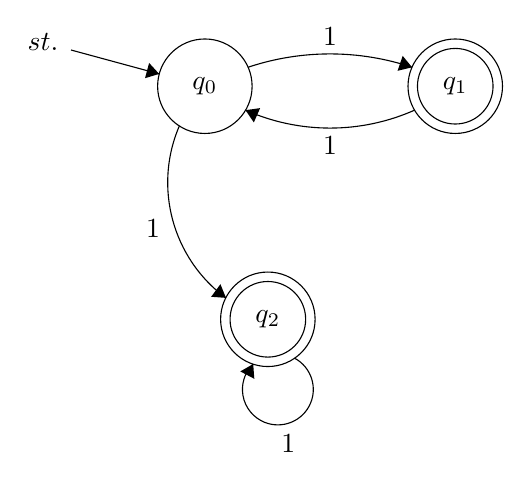
\begin{tikzpicture}[scale=0.2]
\tikzstyle{every node}+=[inner sep=0pt]
\draw [black] (12.6,-28.5) circle (3);
\draw (12.6,-28.5) node {$q_0$};
\draw [black] (28.5,-28.5) circle (3);
\draw (28.5,-28.5) node {$q_1$};
\draw [black] (28.5,-28.5) circle (2.4);
\draw [black] (16.6,-43.3) circle (3);
\draw (16.6,-43.3) node {$q_2$};
\draw [black] (16.6,-43.3) circle (2.4);
\draw [black] (4.1,-26.2) -- (9.7,-27.72);
\draw (3.33,-25.68) node [left] {$st.$};
\fill [black] (9.7,-27.72) -- (9.06,-27.02) -- (8.8,-27.99);
\draw [black] (15.343,-27.295) arc (108.4786:71.5214:16.429);
\fill [black] (25.76,-27.3) -- (25.16,-26.57) -- (24.84,-27.52);
\draw (20.55,-25.95) node [above] {$1$};
\draw [black] (25.92,-30.018) arc (-66.02452:-113.97548:13.216);
\fill [black] (15.18,-30.02) -- (15.71,-30.8) -- (16.11,-29.89);
\draw (20.55,-31.66) node [below] {$1$};
\draw [black] (13.939,-41.945) arc (-126.42784:-203.32414:9.107);
\fill [black] (13.94,-41.94) -- (13.59,-41.07) -- (13,-41.87);
\draw (9.79,-37.51) node [left] {$1$};
\draw [black] (18.288,-45.766) arc (62.1301:-225.8699:2.25);
\draw (17.9,-50.58) node [below] {$1$};
\fill [black] (15.67,-46.14) -- (14.85,-46.61) -- (15.74,-47.08);
\end{tikzpicture}
\end{center}

The string ``11111'' would be accepted, while ``1111'' would be rejected. 
\\\\
\begin{solution}
\indent For the full proof, this problem requires proving both directions of the result.  Let's prove the backwards direction first; assume that a language is described by an All-Paths-NFA $N_A$ (we'll shorten this terminology to APN for this proof).  We need to prove that $N_A$ describes a language that can be represented using a regular expression.  We can construct such a regular expression as follows; working backwards from each final state, construct a regular expression for the string for the current state followed through to a final state.  For example, in the given NFA, we can work backwards from $q_2$ as follows: the expression for $q_2$ itself is $1*$, and the expression for $q_0 \rightarrow q_2$ is $11^*$; similarly, we work backwards from $q_1$: $q_1$ itself has no loops, so the expression for $q_0 \rightarrow q_1$ is given by $(11)^*$.  

Now we have described how to work backwards from final states; what happens when these paths collide while working backwards?  We can just intersect the paths leading to the same state; for example, in the given NFA, the paths $q_0 \rightarrow q_1$ and $q_0 \rightarrow q_2$ intersect at $q_0$ with the expressions $(11)^*$ and $11^*$; here, we can just intersect them to obtain $(11)^* \cup 11^*$ (which is indeed what this NFA describes).  Regular expressions are closed under intersection, so we have constructed some object that can be rewritten properly (using unions and such) as a regular expression.  But since this regular expression describes this APN, we are done with this portion of the proof.

It remains to prove that every regular expression has an .  Take a regular expression; let its language be $L$.  Let the corresponding NFA be $N$.  We claim that turning every non-final and dead state into a final state and turning every final state into a dead state results in an APN (let's call it $N^c$) that accepts $L^c$.  The proof: consider any string $s$ in $L$.  In $N$, there is at least one path for $s$ that ends in a final state.  Consider the same path in $N^c$; note that it now ends in a non-final state, and, since APNs require ALL paths for each string to end in a final state, this particular APN no longer accepts $s$.  This tells us that $N^c$ does not accept any string in $L$.

It remains to prove that $N^c$ accepts every string not in $L$.  Let's take such a string, $s'$.  Note that, in $N$, no path for $s'$ can end in a final state, or $N$ would accept $s'$.  This means that all paths for $s'$ in $N$ end in either a non-final or a dead state.  But in $N^c$, all of these states become final states; this means that $N^c$ accepts $s'$.  Thus, we now know that $N^c$ accepts all of the strings in $L^c$.  But since $L$ and $L^c$ are complements and $N^c$ does not accept $L$, $N^c$ accepts exactly $L^c$.

We can now return to the original problem; take any regular expression, its language $L$, and its NFA, $N$.  It is always possible to construct an NFA for the complement of the regular expression.  Let us do that, and call the new NFA $N'$.  Then $N'$ accepts exactly $L^c$.  Applying the previous process, we can now construct $N'^c$ by flipping every state in $N'$.  The result is an APN that accepts exactly $L$, and we are done.

\end{solution}

\end{document}
